\chapter{Vorbereitung}
\textbf{Versuchsziele}
\begin{itemize}[noitemsep]
	
	\item Funktionalität eines Schutzprüfgerätes kennenlernen
	\item Ablauf von Schutzprüfungen und deren Bedeutung
	\item Bestimmung wichtiger Kennwerte von Schutzrelais
	\item Erstellen eines Prüfprotokolls
	\item Bewertung von Prüfergebnissen
	\item Interpretation von Prüfergebnisse
\end{itemize}

\section{Versuchsvorbereitung - Vorbetrachtungen}
Im folgendem werden die Fragen der Versuchsvorbereitung bearbeitet.

\subsection{Warum muss das Rückfallverhältnis von Schutzrelais bekannt sein?}

Das Rückfallverhältnis ist das Verhältnis von Rückfallwert zu Ansprechwert. Es muss bekannt sein, da damit die Anregesicherheit und somit der Anfang des zulässigen Einstellbereiches der $I>$ Anregung bestimmt wird.

\begin{figure}
	\centering
	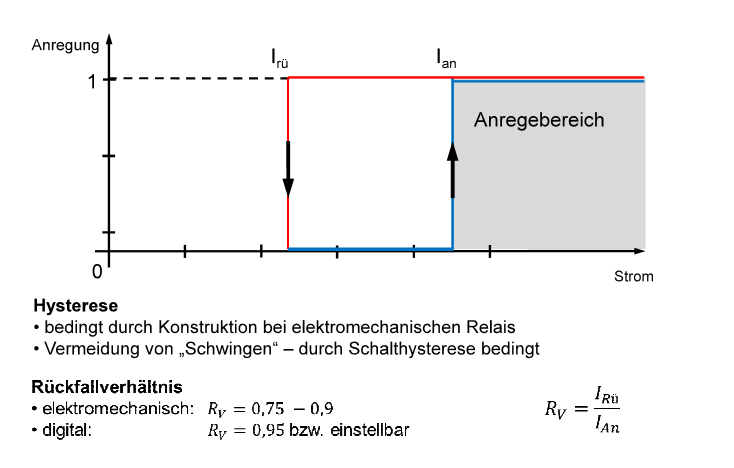
\includegraphics[width=0.7\linewidth]{figures/anregung}
	\caption{Beispiel Überstromanregung}
	\label{fig:anregung}
\end{figure}


Das Rückfallverhältnis $R_v$ berechnet sich damit:

\begin{equation}
	R_v=\frac{I_{\textrm{Rü}}}{I_{An}}
\end{equation}

Berechnung der Anregesicherheit: 
\begin{equation}
	I_{AL}=\frac{I_{\mathrm{zul}}\cdot f_{\textrm{ÜL}}\cdot f_{\mathrm{trans}}}{f_M \cdot R_V \cdot f_s}\approx \frac{I_{zul} \cdot f_{\textrm{ÜL}}}{f_s\cdot R_V}
\end{equation}

\begin{flalign*}
	 I_{\mathrm{zul}}  &\coloneqq \textrm{zulässige Dauerbelastung des Betriebsmittels}&&\\
	 f_{\textrm{ÜL}}  & \coloneqq \textrm{Überlastfaktor (Max. Betriebsstorm im Störfall bzw. } I_\mathrm{zul} &&\\
	 f_\mathbf{trans} & \coloneqq \textrm{Berücksichtigung von Transienten} &&\\
	 R_V & \coloneqq \textrm{Rückfallverhältnis}&&\\
	 f_\mathrm{M} &  \coloneqq \textrm{max. Messfehler }&&\\
	 f_s & \coloneqq \textrm{Sicherheitsfaktor} &&\\
\end{flalign*}

\subsection{Welche Größen muss das Prüfgerät ausgeben und wie müssen diese an das Schutzrelais angeschlossen sein? Fertigen Sie eine Skizze an}

Spannungen, Ströme (o.a. Phasenwinkel, Impedanzen..) und Anrege- und Auslösesignale müssen ausgegeben werden.
Je nachdem, ob nur der Strom oder Strom und Spannung und Leiter-Leiter oder Leiter-Erde-Größen ausgewertet werden sollen, muss das Schutzprüfgerät entsprechend mit dem Schutzrelais verschaltet werden.
Zusätzlich muss ein PC dazu geschaltet, über den die Prüfanforderungen und Darstellung der Ergebnisse erfolgt.

\subsection{Wie kann der Ansprechwert der Überstromstufe eines Schutzrelais einfach und sicher ermittelt werden?}
Es werden Prüfschüsse (Strom und Zeit) kurz vor dem Toleranzband der Überstromstufe gesetzt, wo das Schutzgerät nicht auslösen soll sowie kurz hinter dem Toleranzband, wo es auslösen muss. Wenn nur das Ansprechen getestet werden soll, darf der Fehlerstrom nur kurz anstehen (bzw. nicht so lang, bis es zur Auslösung kommt)
Sobald das Schutzgerät den Strom als Fehlerstrom erkannt und klassifiziert hat, setzt es ein Binärsignal für die Anregung (Ansprechen), das vom Schutzprüfgerät erfasst wird. 

\section{Welche grundlegenden Unterschiede ergeben sich bei der Prüfung von elektromechanischen und digitalen Schutzrelais? Wie wird sich das bei den Ergebnissen des Rückfallverhältnisses darstellen?}
